\section{Shor-Algorithmus}
Im folgenden Kapitel wird der Shor-Algorithmus zur Faktorisierung von Zahlen beschrieben. 
Der Inhalt fokussiert sich auf den Zweck, die Funktionsweise und den Aufbau des Algorithmus. 
Der Aufbau beinhaltet nicht die konkrete Implementierung der Bestandteile des Algorithmus. 
Stattdessen werden die Details bezüglich der Implementierung im nächsten Kapitel behandelt.

\subsection{Zweck}
Der Shor-Algorithmus wurde mit dem spezifischen Ziel entwickelt, 
große zusammengesetzte Zahlen effizient auf Quantencomputern in ihre Primfaktoren zu zerlegen. 
Im Gegensatz zu klassischen Faktorisierungsverfahren, 
die exponentielle Zeit in Anspruch nehmen~\cite{katz2023}, 
ermöglicht Shors Ansatz die Faktorisierung in polynomialer Zeit in Bezug auf die Bitlänge der zu faktorisierenden Zahl~\cite{Shor_1997}. 
Dies stellt eine signifikante Beschleunigung gegenüber den besten bekannten klassischen Faktorisierungsalgorithmen dar. 
Der Shor-Algorithmus bekräftigt somit die These, 
dass Quantencomputer bestimmte Probleme wesentlich schneller lösen können als klassische Rechner.

\subsection{Funktionsweise} \label{Funktionsweise}
Der Shor-Algorithmus kombiniert im Wesentlichen zwei Teilberechnungen, 
eine quantenmechanische und eine klassische, 
um eine zusammengesetzte Zahl \(N\) effizient in ihre Primfaktoren zu zerlegen.

Im quantenmechanischen Teil steht die Bestimmung der Ordnung \(p\) einer Zahl \(a\) 
in der multiplikativen Gruppe modulo \(N\) im Fokus. 
Also berechnet der quantenmechanischen Teil nicht direkt die Primfaktoren der zu faktorisierenden Zahl.
Stattdessen wird die Eigenschaft ausgenutzt, 
dass das Problem der Faktorisierung äquivalent zu dem Problem der Ordnungsbestimmung ist~\cite[226,633]{nielsen_chuang_2010}.
Daher impliziert eine effiziente Lösung für die Berechnung der Ordnung eine ebenso effiziente Methode zur Faktorisierung.

Der nachfolgende klassische Teil des Algorithmus nimmt im Anschluss die ermittelte Ordnung als Eingabe und nutzt sie, 
um die Primfaktoren der Zahl \(N\) abzuleiten.

Beide Teilberechnungen, sowohl der quantenmechanische als auch der klassische Teil, 
benötigen für ihre Berechnungen eine polynomiale Laufzeit. 
Daher ist die gesamte Laufzeit des Shor-Algorithmus ebenfalls von polynomialer Größenordnung.

\subsection{Ordnungsbestimmung} \label{Shor:Ordnungsbestimmung}
Zu bestimmen sind die Primfaktoren der Zahl \(N\).
Zuerst wird ein \(a\) mit \(0 < a < N\) gewählt.
Falls der seltene Fall eintritt, dass \(a\) nicht teilerfremd zu \(N\) ist, entspricht \(a\) einem der Primfaktoren, weswegen 
keine weiteren Berechnungen mehr nötig wären.
Anschließend wird die Ordnung beziehungsweise Periode \(p\) der Funktion \({f(x) = a^x \bmod N}\) mit dem Quantenalgorithmus bestimmt.

Die Periode \(p\) beschreibt die kleinste ganze Zahl mit \({p > 0}\), für die gilt: \({f(p) = 1 \bmod N}\).
Bei einem \(a = 7\) und \(N = 15\) ist dies \(p=4\):
\[
\begin{tabular}{l|llllll}
    x     &     0     &     1       &     2      &      3   &  4 &  5  \\ \hline
    \(7^x \bmod 15\)    &      1     &        7     &       4     &     13     &  1 &  7 
\end{tabular} \longmapsto p = 4
\]

Die quantenmechanische Berechnung im Shor-Algorithmus basiert im Wesentlichen auf der Quantum-Phase-Estimation.
Die Architektur dieser spezifischen Quantum-Phase-Estimation korrespondiert weitgehend mit der in Abschnitt~\ref{Quanten-Phase-Estimation} vorgestellten Struktur.
Hierbei werden speziell für die gegebene Anwendung definierte \(U\)-Gatter eingesetzt.

Für den konkreten Kontext der Periodenberechnung, realisieren die \(U\)-Gatter die Transformation:
\[U\ket{y} = \ket{ay \bmod N}\] 
Die Ausführung der Quantum-Phase-Estimation erfordert die Erzeugung eines Eigenvektors der Transformation \(U\).
Da die Quantum-Phase-Estimation \(\varphi\) aus dem Eigenwert extrahiert, 
darf der Eigenvektor nicht den trivialen Eigenwert 1 besitzen.
Stattdessen ist es notwendig, dass die Periode der Transformation im Eigenwert enthalten ist.

Wie in~\cite[227]{nielsen_chuang_2010} gezeigt wird, gibt es zu \(U\) Eigenvektoren \(\ket{u_s}\), 
mit \(0 \leq s \leq p-1\): 
\[\ket{u_s} =
\frac{1}{\sqrt{p}}
\sum_{k=0}^{p-1} e^{\frac{-2 \pi i s k}{p}\ket{a^k \bmod N}} 
\]
Für \(a=7\) bei \(N=15\) entspricht \(p=4\).
Ein Eigenvektor zu \(s=1\) lautet dann:
\begin{align*}
    U^{\tensor 4}\ket{u_1}_4 &=
    \frac{1}{\sqrt{4}}(
        U^{\tensor 4}\ket{1}_4 + 
        e^{-\frac{2 \pi i}{4}}U^{\tensor 4}\ket{7}_4 + 
        e^{-\frac{4 \pi i}{4}}U^{\tensor 4}\ket{4}_4+ 
        e^{-\frac{6 \pi i}{4}}U^{\tensor 4}\ket{13}_4
    )\\
    &=
    \frac{1}{\sqrt{4}}(
        \ket{7}_4 + 
        e^{-\frac{2 \pi i}{4}}\ket{4}_4 + 
        e^{-\frac{4 \pi i}{4}}\ket{13}_4+ 
        e^{-\frac{6 \pi i}{4}}\ket{1}_4
    )\\
    &=
    e^{\frac{2 \pi i}{4}}
    \cdot
    \frac{1}{\sqrt{4}}(
        e^{-\frac{2 \pi i}{4}}\ket{7}_4 + 
        e^{-\frac{4 \pi i}{4}}\ket{4}_4 + 
        e^{-\frac{6 \pi i}{4}}\ket{13}_4+ 
        e^{-\frac{8 \pi i}{4}}\ket{1}_4
    )
\end{align*}
Durch Substition mit
\begin{align*}
    \ket{u_1}_4 &=
    \frac{1}{\sqrt{4}}(
        \ket{1}_4 + 
        e^{-\frac{2 \pi i}{4}}\ket{7}_4 + 
        e^{-\frac{4 \pi i}{4}}\ket{4}_4+ 
        e^{-\frac{6 \pi i}{4}}\ket{13}_4
    )
\end{align*}
erhält man schlussendlich:
\begin{align*}
    U^{\tensor 4}\ket{u_1}_4 
    =e^{\frac{2 \pi i}{4}} \cdot
    \ket{u_1}_4
\end{align*}
Das kann verallgemeinert werden:
\[U\ket{u_s} = e^{\frac{2 \pi i s}{p}}\ket{u_s}\]

Wie man in der Definition von \(\ket{u_s}\) 
sieht, 
benötigt die Initialisierung eines Eigenvektors \(\ket{u_s}\) mit einem konkreten \(s\) die Periode \(p\).
Man kann diese Problematik jedoch umgehen indem man anstelle eines einzelnen Eigenvektors \(\ket{u_s}\)
eine Superposition verwendet, die alle \(\ket{u_s}\) umfasst.
Die Superposition entspricht~\autocite[227]{nielsen_chuang_2010}:
\[\frac{1}{\sqrt{p}} \sum_{s=0}^{p-1}\ket{u_s} = \ket{1}\] 
Daher wird das Qubit, welches das Least-Significant-Bit des Qubit-Registers für den Eigenvektor darstellt, 
mit dem Zustand \(\ket{1}\) initialisiert.

Die Superposition der Eigenvektoren hat zur Folge, 
dass nach der inversen Quanten-Fourier-Transformation, also am Ende der Quantum-Phase-Estimation,
ebenfalls eine Superposition mit dem \(\varphi_s\) der Eigenwerte \(\lambda_{u_s}\) aller möglichen Eigenvektoren \(\ket{u_s}\) existiert.
Sei \(k\) die Anzahl der Kontrollqubits. 
Dann nehmen diese den folgenden Zustand an:
\[
    \frac{1}{\sqrt{p}} \sum_{s=0}^{p-1}\ket{2^k \cdot \frac{s}{p}}_k   = 
    \frac{1}{\sqrt{p}} \Bigg(\ket{0}_k  + \ket{2^k \cdot \frac{1}{p}}_k + \ket{2^k \cdot \frac{2}{p}}_k  \dotsb + \ket{2^k \cdot \frac{p-1}{p}}_k \Bigg)
\]
Bei einer Messung wird also zufällig eines der insgesamt \(p\) vielen \(\varphi_s = \frac{s}{p}\) gemessen.

Die Genauigkeit des Algorithmus, ausgedrückt durch den Parameter \(k\),
ist direkt abhängig von der Anzahl der verwendeten \(U^{2^x}\)-Gatter
und der damit assoziierten Kontrollqubits im Quantenschaltkreis.
Somit definiert \(k\) die Genauigkeit des Messwertes gegenüber dem \(\varphi_s\).

Wenn genügend Kontrollqubits verwendet werden, 
wird bei einer Messung ein Zustand gemessen, 
in dem \(\varphi_s\) beziehungsweise \(\frac{s}{p}\) enthalten ist.

Falls nicht ausreichend Kontrollqubits vorhanden sind 
und der Wert von \(\varphi_s\) somit nicht ausreichend umfasst werden kann,
wird die Messung mit hoher Wahrscheinlichkeit 
in einen der möglichen Zustände kollabieren, 
der dem genauen Ergebnis am nächsten ist.
Dadurch bildet sich ein Peak rund um den korrekten Wert, 
der vergleichbar ist mit Abbildung~\ref{fig:3_qubit_qpe_measurment_uncertain}.
Genau wie in Abbildung~\ref{fig:3_qubit_qpe_measurment_uncertain}, haben die Werte nah dem genauen Wert
eine höhere Chance gemessen zu werden. 
Konkret ist die Wahrscheinlichkeit, 
einen der direkten ganzzahligen Nachbarn des genauen Ergebnisses zu erhalten, 
größer als \(\frac{8}{\pi^2}\)~\cite[119]{kaye2007introduction}.
Da aber eine Messung von probabilistischer Natur ist, 
kann eine Messung auch zu einem Ergebnis führen, 
welches entfernt vom genauen Ergebnis liegt.
Selbst wenn der gemessene Wert dem bestmöglichen Ergebnis entspricht, 
kann dieser von \(\frac{s}{p}\) abweichen. 

Anders als in Abbildung~\ref{fig:3_qubit_qpe_measurment_uncertain} gibt es bei der Periodenbestimmung insgesamt \(p\) Peaks.
Das liegt daran, dass es insgesamt \(p\) viele Zustände in der Superposition des Endzustandes gibt.

Anhand des Messergebnisses erfolgt die Primfaktorzerlegung in einer Nachberechnung.

\subsection{Klassische Nachberechnung} \label{Funktionsweise:klassisch}
Die Nachberechnung benötigt keine Quantenbrechnung und 
wird daher mit einem klassischen Algorithmus durchgeführt.

Ein einzelner Zustand der finalen Superposition 
entspricht einem genauen Ergebnis und hat die Form \(\ket{2^k \cdot \frac{s}{p}}_k\) für \(0 \leq s < p\).
Indem eine Division durch \(2^k\) durchgeführt wird, kann \(\frac{s}{p}\) extrahiert werden.
Als Beispiel sei die finale Superposition für \(a = 7;~N=15\) mit \(p=4\) und einer Genauigkeit von \(k=4\) gegeben:
\[\frac{1}{\sqrt{4}}
\Bigg(\ket{0}_4 +\ket{2^4 \cdot \frac{1}{4}}_4 + \ket{2^4 \cdot \frac{2}{4}}_4+\ket{2^4 \cdot \frac{3}{4}}_4
\Bigg) =
 \frac{1}{\sqrt{4}}
 \Big(\ket{0}_4 +\ket{4}_4 + \ket{8}_4+\ket{12}_4\Big) \]
Mit Ausnahme der Zustände \(\ket{0}_4\) und \(\ket{8}_4\) 
resultieren die beiden anderen Zustände nach einer Division durch \(2^4\) in einer Kommazahl. 
Diese kann als Bruch dargestellt werden, 
dessen Nenner die gesuchte Periode \(p=4\) ist.

Im vorherigen Beispiel handelt es sich bei der Periode um eine 2er Potenz, 
deshalb sind die genauen Zustände ganzzahlig und die Messergebnisse somit eindeutig.
Dies ist jedoch ein ideales Szenario, 
das bei immer größeren \(N\) seltener auftritt. 
Das nächste Beispiel beachtet \(a=11;~N=21\) mit der Periode \(p=6\) und einer Genauigkeit von \(k=4\):
\[\frac{1}{\sqrt{6}}
\Bigg(\ket{0}_4 +\ket{2^4 \cdot \frac{1}{6}}_4 + \ket{2^4 \cdot \frac{2}{6}}_4+
\ket{2^4 \cdot \frac{3}{6}}_4+\ket{2^4 \cdot \frac{4}{6}}_4 + \ket{2^4 \cdot \frac{5}{6}}_4
\Bigg) \]
\[= \frac{1}{\sqrt{6}}
\Big(\ket{0}_4 +\ket{2,\overline{6}}_4 + \ket{5,\overline{3}}_4+
\ket{8}_4+\ket{10,\overline{6}}_4 + \ket{13,\overline{3}}_4
\Big) \]
Die Kontrollqubits, welche gemessen werden, 
können keine Kommazahlen darstellen.
Infolgedessen bildet sich um die benachbarten Zustände eine Wahrscheinlichkeitsverteilung, 
die bei dem ganzzahligen Zustand, der am nächsten liegt, 
ihren Höhepunkt hat, vergleichbar mit Abbildung~\ref{fig:3_qubit_qpe_measurment_uncertain}.
Im konkreten Beispiel wird für \(\ket{2,\overline{6}}_4\) der Zustand \(\ket{3}_4\) 
mit der höchsten Wahrscheinlichkeit gemessen.
Eine Extraktion der Periode aus \(\ket{3}_4\) mit einer Division durch \(2^4\) liefert als Ergebnis die Kommazahl \(0,1875\).
Um von dieser Kommazahl den nächsten Bruch zu finden, wird der Kettenbruch-Algorithmus angewendet.
Im konkreten Fall wird dadurch \(\frac{3}{16}\) gefunden.
Der Bruch \(\frac{3}{16}\) enthält im Nenner nicht die gesuchte Periode \(p=6\). 
Das Gleiche gilt auch für andere Zustände, 
die mit hoher Wahrscheinlichkeit gemessen werden können, wie 
\(\ket{5}_4,~\ket{8}_4,~\ket{11}_4\) und \(\ket{13}_4\).

Das Scheitern der vorangegangenen Berechnung ist auf eine unzureichende Genauigkeit zurückzuführen. 
In der vorangegangenen Darstellung werden \(k=4\) Kontrollqubits eingesetzt, 
welche für die gesuchte Periode einen zu kleinen Wertebereich bilden.

Wird das Verfahren mit \(k=7\) wiederholt, ergibt sich die folgende Superposition:
\[\frac{1}{\sqrt{6}}
\Big(\ket{0}_7 +\ket{21,\overline{3}}_7 + \ket{42,\overline{6}}_7+
\ket{64}_7+\ket{85,\overline{3}}_7 + \ket{106,\overline{6}}_7
\Big) \]
Es ist ersichtlich, dass die genauen Zustände immer noch Nachkommastellen aufweisen, 
weshalb mit einer geringeren Wahrscheinlichkeit auch andere Werte gemessen werden können.
Bei einer Messung ist anstelle des Zustands \(\ket{21,\overline{3}}_7\) der Zustand \(\ket{21}_7\) das Ergebnismit der höchsten Wahrscheinlichkeit .
Für \(\frac{21}{2^{7}}\) erhält man eine Kommazahl, deren exakter Bruch \(\frac{21}{128}\) entspricht.
Wendet man den Kettenbruch-Algorithmus auf \(\frac{21}{128}\) an und limitiert den Nenner auf \(N\), 
wird der nächstgelegene Bruch mit einem Nenner gefunden, der kleiner als \(N\) ist.
Der Nenner wird auf \(N\) limitiert, da die Periode einer Zahl \(p\) entspricht die kleiner ist als \(N\).
Im konkreten Beispiel ergibt sich aus \(\frac{21}{128}\) der Bruch \(\frac{1}{6}\), 
welcher die Periode im Nenner offenbart.
Bei einer Messung könnte auch der benachbarte ganzzahlige Zustand \(\ket{22}_7\) gemessen werden, 
allerdings mit einer geringeren Wahrscheinlichkeit im Vergleich zu \(\ket{21}_7\).
Der Zustand \(\ket{22}_7\) ermöglicht nicht die Extraktion der Periode, 
da \(\frac{22}{128}\) mit dem Kettenbruch-Algorithmus auf einen für \(N\) limitierten Nenner
zu \(\frac{3}{17}\) wird.

Das bedeutet, 
mit einer hinreichenden Genauigkeit, kann die Periode nur aus dem Zustand extrahiert werden, 
welcher den Wert des genauen Zustandes am besten approximiert.

Mit zusätzlichen Kontrollqubits wird das Messergebnis fehlertolerant.
Wiederholt man das Beispiel erneut, diesmal jedoch mit \(k=10\), 
ist der zweite Zustand in der finalen Superposition: 
\(\ket{2^{10} \cdot \frac{1}{6}}_{10} =\ket{170,\overline{6}}_{10}\).
Im Gegensatz zu vorher liefert jetzt nicht nur das am besten approximierte Ergebnis, 
in dem Fall die \(\ket{170}_{10}\), mit dem Kettenbruch-Algorithmus die Periode, 
sondern auch alle benachbarten Zustände von \(\ket{167}_{10}\) bis \(\ket{175}_{10}\).

Durch den Einsatz von zusätzlichen Kontrollqubits erhöht sich der Wertebereich. 
Aufgrund des größeren Wertebereiches existieren mehr mögliche Zustände, 
die bei einer Messung vorkommen könnten und ebenfalls auch mehr Zustände, 
die die Extraktion der korrekten Periode ermöglichen. 
Dabei ist die Wahrscheinlichkeitsverteilung der ausschlaggebende Faktor. 
Diese verändert sich mit einer wachsenden Anzahl an Kontrollqubits zugunsten der Zustände, 
welche die korrekte Periode offenbaren.
Die Abbildungen~\ref{fig:Messung7k} und~\ref{fig:Messung10k} 
heben den Effekt zusätzlicher Kontrollqubits auf die Wahrscheinlichkeitsverteilung der Messungen hervor.
Die grünen Säulen im Diagram zeigen die Messergebnisse, 
welche nach der Anwendung des Kettenbruch-Algorithmus die Periode enthalten.

\begin{figure}[H]
    \centering
    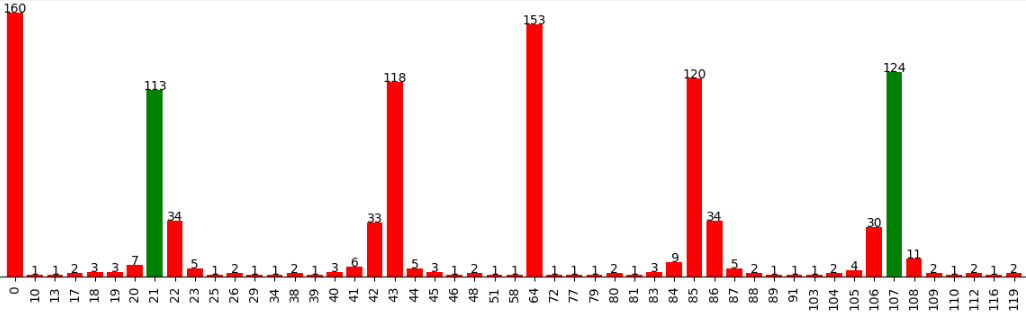
\includegraphics[scale = 0.55]{wahrscheinlichkeit_k7.PNG}
    \caption{Messergebnisse für a=11, N=21, k=7 bei 1024 Messungen}
    \label{fig:Messung7k}
\end{figure}
\begin{figure}[H]
    \centering
    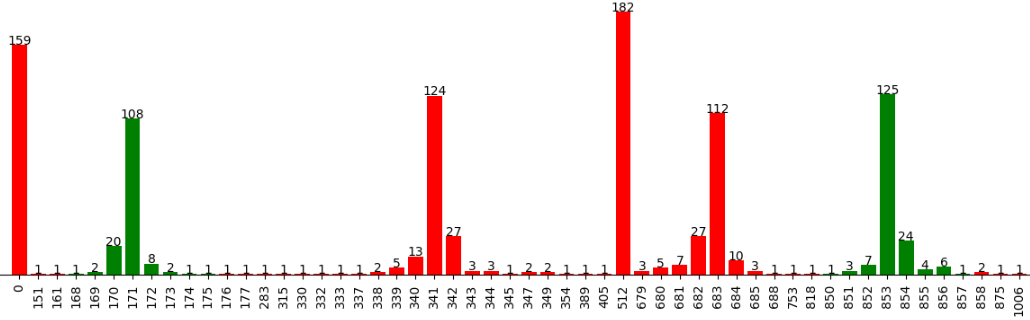
\includegraphics[scale = 0.55]{wahrscheinlichkeit_k10.PNG}
    \caption{Messergebnisse für a=11, N=21, k=10 bei 1024 Messungen}
    \label{fig:Messung10k}
\end{figure}

Es lässt sich zeigen, dass bei einer bekannten Periode \(p\) die Wahl von \(k > 2\ld(p)\) 
eine ausreichende Genauigkeit gewährleistet. 
Unter diesen Bedingungen wird eines der bestmöglichen Messergebnisse durch den Einsatz des Kettenbruch-Algorithmus zu einem Näherungsbruch \(\frac{s}{p}\) von \(\varphi_s\) konvergieren.
Im Normalfall kann für ein Element \(a\) für den Modulus \(N\) vorab nicht gesagt werden, 
wie viele Kontrollqubits man exakt braucht, 
da dies von der unbekannten Periode \(p\) abhängt.
Stattdessen verwendet man einen Wert der auf alle Fälle größer als \(2\ld(p)\) ist, 
wie zum Beispiel \(2\ld(N)\).~\cite{Shor_1997,mosca1999hidden}

Wie man in Abbildungen~\ref{fig:Messung10k} sieht, 
gibt es auch bei der Verwendung von \(2\ld(N)\) Kontrollqubits einige Messergebnisse, 
bei denen ein Zustand mit einer ungültigen Periode gemessen werden kann.
Diese Zustände lassen sich in drei Szenarien oder Fallunterscheidungen einteilen:

Im Falle des ersten Szenarios 
entspricht mindestens einer der Zustände der finalen Superposition einer Kommazahl.
Dadurch können Messungen von falschen Werten auftreten.
Anhand eines solchen Ergebnisses führt die Anwendung des Kettenbruch-Algorithmus nicht zu \(\frac{s}{p}\), 
weswegen eine neue Messung benötigt wird.

Das zweite Szenario ähnelt dem ersten und tritt ebenfalls auf, 
sobald mindestens einer der Zustände der finalen Superposition eine Kommazahl ist. 
Im Unterschied zum ersten Szenario liegt dieses Messergebnis jedoch nah bei einem Peak, 
also in der Nähe eines Messergebnisses, aus dem die Periode extrahiert werden kann. 
Indem man die Nachbarzustände des Messergebnisses testet, kann man gegebenenfalls einen Zustand finden, 
der die Extraktion der Periode ermöglicht.

Beispielsweise tritt das zweite Szenario bei dem Messergebnis \(\ket{176}_{10}\) in Abbildung~\ref{fig:Messung10k} auf.
Die Anwendung des Kettenbruch-Algorithmus auf \(\frac{176}{2^{10}}\) 
liefert nicht die korrekte Periode, stattdessen ergibt sich der Bruch \(\frac{3}{17}\). 
Anstatt eine neue Messung durchzuführen,
ist es in diesem Fall zielführend, 
die ganzzahligen Nachbarn des Messergebnisses zu überprüfen.
Im konkreten Beispiel ermöglicht bereits die geringfügige Anpassung des Messergebnisses durch Subtraktion von 1, 
also zu \(\ket{175}_{10}\), 
die erfolgreiche Extraktion der Periode.

Die Erhöhung der Genauigkeit \(k\) auf Werte über \(2\ld(N)\) hinaus hat den Effekt, 
dass die Wahrscheinlichkeit für das Eintreten des ersten oder zweiten Falls abnimmt.
Dadurch verbessert sich gleichzeitig die Wahrscheinlichkeit, direkt ein korrektes Ergebnis zu messen.
Allerdings führt dies zu einem komplexeren Quantenschaltkreis und 
somit erhöhen sich die Kosten an zusätzlichen Ressourcen~\autocite[229]{nielsen_chuang_2010}.

Der dritte und letzte Fall kann immer auftreten.
In diesem Szenario wird ein \(\frac{s'}{p'}\) gemessen, 
welches entsteht, wenn \(s\) und \(p\) einen gemeinsamen Teiler haben und 
deswegen von \(\frac{s}{p}\) auf \(\frac{s'}{p'}\) gekürzt wurden.
In diesem Fall kann ein vielfaches von \(p'\), also \(2p'\),\(3p'\),.. zum richtigen \(p\) führen.
Des Weiteren besteht die Möglichkeit, 
dass bei einer zweiten Messung erneut ein gekürztes \(\frac{s}{p}\) als \(\frac{s''}{p''}\) gefunden wird.
Es ist möglich, dass aus dem kleinsten gemeinsamen Vielfachen von \(p'\) und \(p''\) das \(p\) berechnet werden kann~\cite{Shor_1997}.
Dies ist nur der Fall, wenn \(s'\) und \(s''\) keine Faktoren teilen und 
führt mit einer Wahrscheinlichkeit größer als \(0.25\) zur korrekten Periode \(p\)~\autocite[231]{nielsen_chuang_2010}.

In Abbildung~\ref{fig:Messung10k} sind die beiden Peaks um die Zustände \(\ket{341}_{10}\) und \(\ket{683}_{10}\) rot gefärbt, 
was auf den dritten Fall zurückzuführen ist.
Sowohl \(\ket{341}_{10}\) als auch \(\ket{683}_{10}\) und ihre benachbarten Zustände 
enthalten ursprünglich im Nenner die korrekte Periode, 
wurden jedoch  auf \(\frac{1}{3}\), beziehungsweise \(\frac{2}{3}\), gekürzt. 
Eine Überprüfung der nächsten Vielfachen, in diesem Fall \(2 \cdot 3 = 6 \), führt zur korrekten Periode.

Es lässt sich zeigen, dass die Wahrscheinlichkeit mindestens \(\frac{1}{2\ld(N)}\) beträgt, 
bei einer Messung ein \(s\) zu erhalten, welches eine Primzahl ist und somit zu \(p\) teilerfremd ist.
Das bedeutet, dass die Wahrscheinlichkeit bei insgesamt \(2\ld(N)\) Messungen sehr hoch ist, 
mindestens einmal ein \(\frac{s}{p}\) zu messen, 
bei dem \(s\) und \(p\) nicht gekürzt sind.~\cite[231]{nielsen_chuang_2010}

Ob die korrekte Periode gefunden wurde, kann mit \(a^p = 1 \bmod N\) geprüft werden.

Sobald die korrekte Periode \(p\) gefunden wurde, 
können die Primfaktoren von \(N\) mit dem größten gemeinsamen Teiler (\(\gcd\)) berechnet werden:
\[\gcd(a^{\frac{p}{2}}-1, N), \gcd(a^{\frac{p}{2}}+1, N)\]
Dies schlägt nur fehl, 
wenn \(p\) ungerade ist
oder wenn \(a^{\frac{p}{2}} = -1 \bmod N\) erfüllt ist.
Die Wahrscheinlichkeit, dass einer der beiden genannten Fälle eintritt, beträgt \(1-\frac{1}{2^f}\), 
wobei \(f\) die Anzahl an unterschiedlichen Primfaktoren von \(N\) angibt.
In einem solchen Fall wiederholt man die Periodenberechnung mit einem anderen \(a\).~\cite{Shor_1997}

